\subsection{Test vehicle description}
\label{sec:test-vehicle-desc}

% A testchip has been made to put measurement structures on silicon
Integrated circuits are very dense and fragile devices, enclosed in plastic or ceramic packages.
It is nearly impossible to measure electrical properties without physical access.
For instance, it could be useful to measure potential inside a given net inside the circuit.
With integrated circuits, this is not doable and most of the time the external connections are the only points of access.
Even with physical internal access, placing micro-probes to contact metal connections can disturb sensitive parts of the device.
To overcome these issues, new approaches are required.
In this research, custom measurement structures have been implemented directly on-chip.
They perform analog measurements at the silicon level.

\begin{figure}[h]
  \centering
  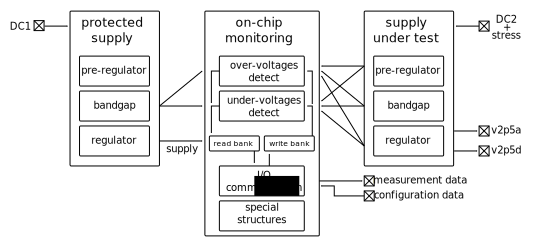
\includegraphics{src/3/figures/architecture_testchip.pdf}
  \caption{Global architecture of the test vehicle}
  \label{architecture_testchip}
\end{figure}

The global architecture of the testchip is provided in Fig. \ref{architecture_testchip}.
It contains two instances of the regulation function studied earlier in \ref{sec:study-real-product}.

% Right supply
The first instance (right side of Fig. \ref{architecture_testchip}) is exposed to \gls{ESD} stresses during tests.
It is monitored in multiple points by the measurement and monitoring structures.

% Left supply
The second instance powers the monitoring functions and communication buses.
It must not be disturbed by the discharges injected during testing on DC\textsubscript{2}.
It has its own external supply pin DC\textsubscript{1}, isolated from DC\textsubscript{2}.
Large external filtering and decoupling capability has been setup on DC\textsubscript{1}.
Except for the ground connection, the two regulators do not share connections.

% What is in the monitoring system
The on-chip monitoring system is composed of several overvoltage and undervoltage detectors.
They monitor voltages of multiple nets inside the supply under test.
There are in total 9 detectors in the testchip.
5 of them are dedicated to preliminary testing and self-validation, and are not actually monitoring analog blocks.
The 4 remaining blocks are monitoring the regulator under test (Table \ref{tab:detectors}).
Threshold can be configured externally using a communication bus.
When new value is set through the communication, a digital to analog converter generates the new threshold for each detector.
The detectors are able to detect level crossings from half a volt up to 13 V, which is designed to match the voltage range of most signals inside the chip.

\begin{table}[!htbp]
\centering
\begin{tabular}{@{}lll@{}}
\toprule
Name           & Nominal value & Function \\ \toprule
uv\_9V	       & 9V   & undervoltage detect on v\textsubscript{clamp9} (settable threshold)\\
ov\_9V	       & 9V   & overvoltage detect on v\textsubscript{clamp9} (settable threshold)\\
ov\_vref1p2	   & 1.2V & overvoltage detect on bandgap reference (settable threshold) \\
uv\_vref1p2	   & 1.2V & undervoltage detect on bandgap reference (settable threshold) \\
\bottomrule
\end{tabular}
\caption{Detectors on core functions}
\label{tab:detectors}
\end{table}

% What is in the communication system
The communication buses provide a connection between the internal detectors and the external world, using digital \gls{io}.
Configuration data can be provided from an external microcontroller and measurement data is output by the communication block.
There are two readable buses and two writeable buses.
The first read and write buses are used for preliminary validation of the on-chip monitoring.
The complete register maps in read and write mode are given in appendix \ref{apx:testchip-register-maps}.

% How those monitoring functions have been designed
The implementation of each monitoring function is detailed hereafter.

\subsection{Voltage monitoring}

% What are the OV/UV detectors made of
Overvoltage and undervoltage detectors are built with latched comparators.
A flag is raised if a monitored net crosses a threshold, and stored using a latch, until it can be read.
The architecture of a single detector is given Fig. \ref{fig:architecture-ov}.
The same architecture is used for the overvoltage and the undervoltage.
Monitored and reference inputs are just inversed on the undervoltage detector.

\begin{figure}[!h]
  \centering
  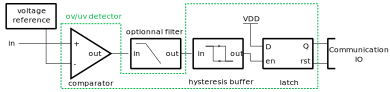
\includegraphics[width=0.9\textwidth]{src/3/figures/architecture_OV.pdf}
  \caption{Architecture of the overvoltage detector}
  \label{fig:architecture-ov}
\end{figure}

% Detail architecture
The first block in this detector is the comparator.
It is designed with a two-stage operational amplifier with an output buffer (see Fig. \ref{fig:comparator-design}).
This topology is well suited for high-gain, open-loop comparators.
This comparator provides a very high input impedance, to ensure the monitored net is not disturbed.
A high-gain is useful for limiting the comparator's offset and to ensure that the comparison will be accurate.
The offset of the designed comparator is below 5 mV and the switching speed under 20 ns (on a 50pF load), which should be sufficient to detect fast glitches of several volts amplitude and a timescale similar to electrostatic discharges.

\begin{figure}[!h]
  \centering
  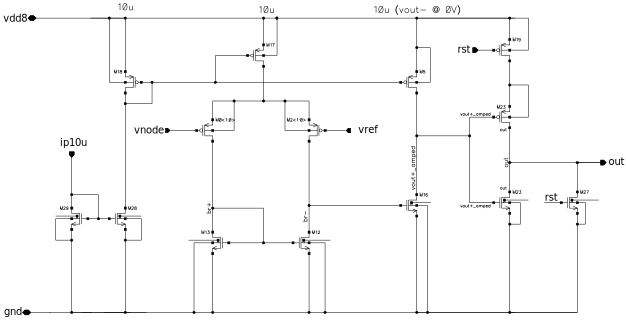
\includegraphics[width=0.9\textwidth]{src/3/figures/comparator_design_clean.pdf}
  \caption{Comparator design}
  \label{fig:comparator-design}
\end{figure}

% What is the purpose of filter
On the output of the comparator (Fig. \ref{fig:architecture-ov}), an optional RC filter can be connected.
This filter can deglitch very short overvoltages, to only let large overvoltages pass through the detector.
The stratety behind this filter is to use multiple detectors monitoring the same net, each one with a different filter.
In function of which detectors triggered, an estimation of the overvoltage length can be made.

% Hysteresis buffer
After the filter, an hysteresis buffer guarantees that a clean digital signal will be fed to the latch.
The triggering levels are set quite far away, with the low level near 2V and the high level at about 6V.

% Latch
Finally, the latch stores the overvoltage flag.
By default it stores a low-level.
Its copy input $D$ is connected to the supply.
If the hysteresis buffer triggers high, the enable pin triggers a copy in the latch.
The output $Q$ copies the value from the $D$, storing a logical high in the latch.
This way, any detected overvoltage or undervoltage is stored until it can be red or the latch is reset.

% Origin of reference voltages
The reference voltages for these comparators come from either fixed-values set by the protected supply, or \gls{dac} that can be reconfigured through the communication system.

\subsection{Communication system}
\label{sec:comm-system-testchip}

% Why a comm IO
The manufacturing process at NXP for test vehicles requires a 48 pin package.
On those 48 pins, a few are already required for ground connection and substrate connection.
Also, the two instances of the regulation function each need a supply connection and two external decoupling capacitors.
The on-chip current sensor also require 4 pins for the calibration pattern and two pins per actual sensor.
In the end, the available pin count would be too small for allowing to connect each detector to its own external pin.
To overcome this issue, a custom communication bus has been designed, to discuss with the testchip before and after ESD tests.
Initially, the JTAG (Joint Test Action Group) \cite{jtag} protocol was envisionned for this application.
It is a test port for access and boundary-scan.
It is commonly used to check that connections are correct between integrated circuits, and to configure internal parameters such as trim values and internal fuses.
However, the JTAG system needs a digital state-machine for operation, described in any hardware description language (HDL).
This step requires digital-synthesis, a step that converts a HDL sources into electrical netlist.
Given the resource constraints in this research work, this step was not available for this test vehicle.
Instead, a simplified serial to parallel protocol has been designed from scratch.
The main idea to design reusable communication cells that can be duplicated and connected in a chain fashion, to get a register map of any size easily.
Changing the size of the register is simply a matter of adding or removing individual cells.
No digital-synthesis is being required.

% Overall architecture
The chain of individual cells functions by propagating from cell to cell an enable signal.
Each time a cell receives the enable signal, it will perform its task, then pass the enable to the next cell at the next clock edge.

\subsubsection{Read cell}

% Explain behavior
The read cell is constituted of a tri-state buffer and a D-latch (see Fig. \ref{fig:read-cell-design}).
The output of the tri-state buffer is set in high-impedance when input \textit{x} is low.
This action releases the communication bus for other read cells and is the default state.

\begin{figure}[!h]
  \centering
  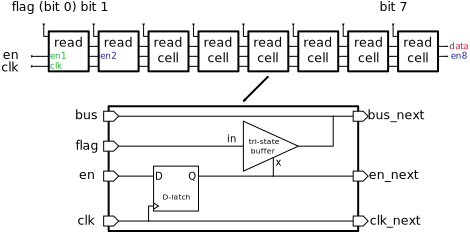
\includegraphics[width=0.8\textwidth]{src/3/figures/architecture_read_cell.pdf}
  \caption{Read-only cell design}
  \label{fig:read-cell-design}
\end{figure}

% Describe the chronogram
Fig. \ref{fig:read-cell-curve} shows the simulated behavior of a chain of 8 reading cells.
Signals in green (\textit{en1} and \textit{clk}) must be provided externally, by a microcontroller for instance.
Signals in blue (\textit{en2} and \textit{en8}) are internal control signals, to help the cells determine if they have the right to write on the bus.
The signal in red (\textit{data}) is the data output, read by an external microcontroller.

% Explain time-response
The reading sequence is initiated by setting \textit{en1} high.
When \textit{en1} is set high, the output of the first latch (\textit{en2}) switches high at the next clock cycle.
This means the first cell has the permission to write on the bus.
During one clock cycle, the \textit{flag} is written on \textit{data} bus.
At the next clock cycle, the enable signal is propagated to the next cell.
The first cell no longer has the permission to write to the bus.
The second cell writes to the bus, during a single clock cycle.
The process is naturally repeated by the system, until the enable has been propagated to the last cell (\textit{en8}) and all serial data was written.

\begin{figure}[!h]
  \centering
  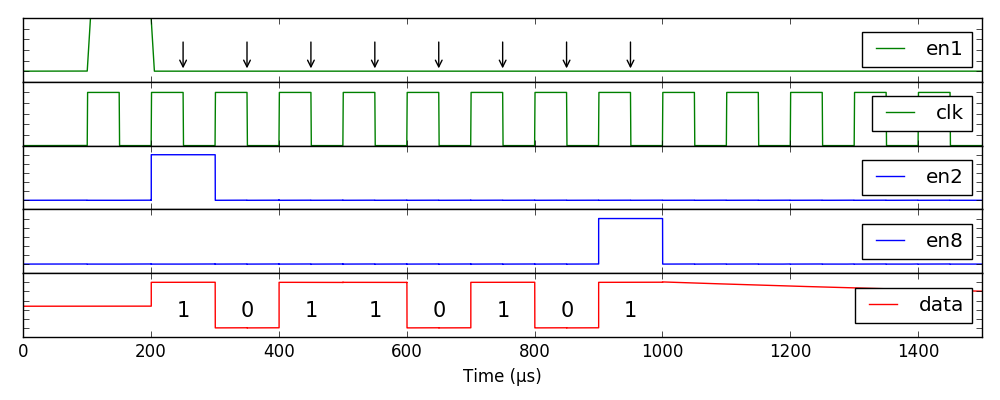
\includegraphics[width=0.95\textwidth]{src/3/figures/curve_read_cell.png}
  \caption{Chronogram for the read cell}
  \label{fig:read-cell-curve}
\end{figure}

\subsubsection{Write cell}

% Explain behavior
The write cell is a bit more complex but operates on the same principle (Fig. \ref{fig:write-cell-design}).
Data is placed serially by the user on the \textit{bus} line, syncronously with the clock.
The enable signal is propagated from cell to cell, so that each cell knows when to sample the bus line and store the value.
Basically, this cell sets on its \textit{output} the value on the bus when its enable is high (Fig. \ref{fig:write-cell-curve}).

\begin{figure}[!h]
  \centering
  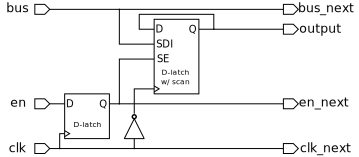
\includegraphics[width=0.8\textwidth]{src/3/figures/architecture_write_cell.pdf}
  \caption{Write-only cell design}
  \label{fig:write-cell-design}
\end{figure}

% Detail devices
The truth table of this latch is given in table \ref{tab:d-latch-scan-truth}.
D1 is a synchronous D-latch.
The output Q copies the input D on rising clock edges.
D2 is a synchronous D-latch with scan.
The output Q copies the data input D on rising clock edges, storing a value.
When the scan enable \textit{se} input is HIGH, the data input D copies the value of the scan data input (\textit{SDI}), effectively changing the stored value.

\begin{table}[!h]
\centering
\begin{tabular}{@{}lllll@{}}
\toprule
D  &  SDI  &  SE  &  CLK  &  Q \\ \midrule
0  &  -    &  0   &  \nearrow    &  0 \\
1  &  -    &  0   &  \nearrow    &  1 \\
-  &  0    &  1   &  \nearrow    &  0 \\
-  &  1    &  1   &  \nearrow    &  1 \\
-  &  -    &  -   &  \searrow    &  Q \\
\bottomrule
\end{tabular}
\caption{D-latch with scan truth-table}
\label{tab:d-latch-scan-truth}
\end{table}

\begin{figure}[!h]
  \centering
  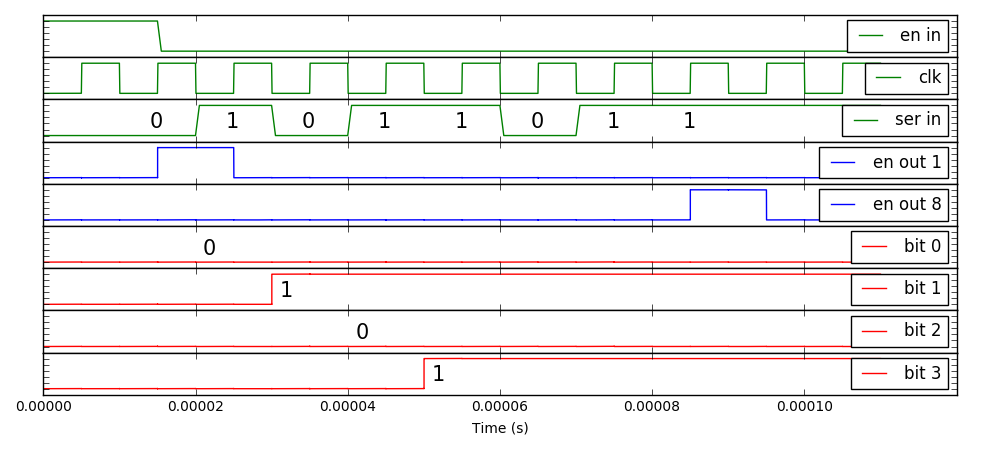
\includegraphics[width=0.95\textwidth]{src/3/figures/curve_write_cell.png}
  \caption{Chronogram for the write cell}
  \label{fig:write-cell-curve}
\end{figure}

% Describe the chronogram
Fig. \ref{fig:write-cell-curve} shows the simulated behavior of a chain of 8 writing cells.
Signals in green (\textit{en1} and \textit{clk}) must be provided externally.
Signals in blue are internal control signals, to help the cells determine if to who belongs the data on the bus.
The signals in red (\textit{bit 0} to \textit{bit n}) are the data output, set on each individual output bit.
Ultimately, the reading-cell performs a serial to parallel conversion.
The serial data is set on \textit{bus}, and the parallel outputs are \textit{bit 0} to \textit{bit n}.

\subsection{On-chip near-field current sensors}

% Measuring currents is important too
Current sensing magnetic loops were integrated on silicon to measure current trough a few critical nets.
They are sensitive to currents circulating nearby, and were placed close to metal tracks in which current must be measured.
By coupling, the sensor generates a voltage proportional to the derivative of the current in the track.
Figs. \ref{fig:near-field-current-sensor} and \ref{fig:near-field-current-sensor-layout} give respectively a visual representation of the metallic loop and its layout.
This kind of integrated loop was studied in \cite{OtherInductors, InductorsLAAS1, InductorsLAAS2, AlainSallesInductors}.

\begin{figure}[!h]
  \centering
  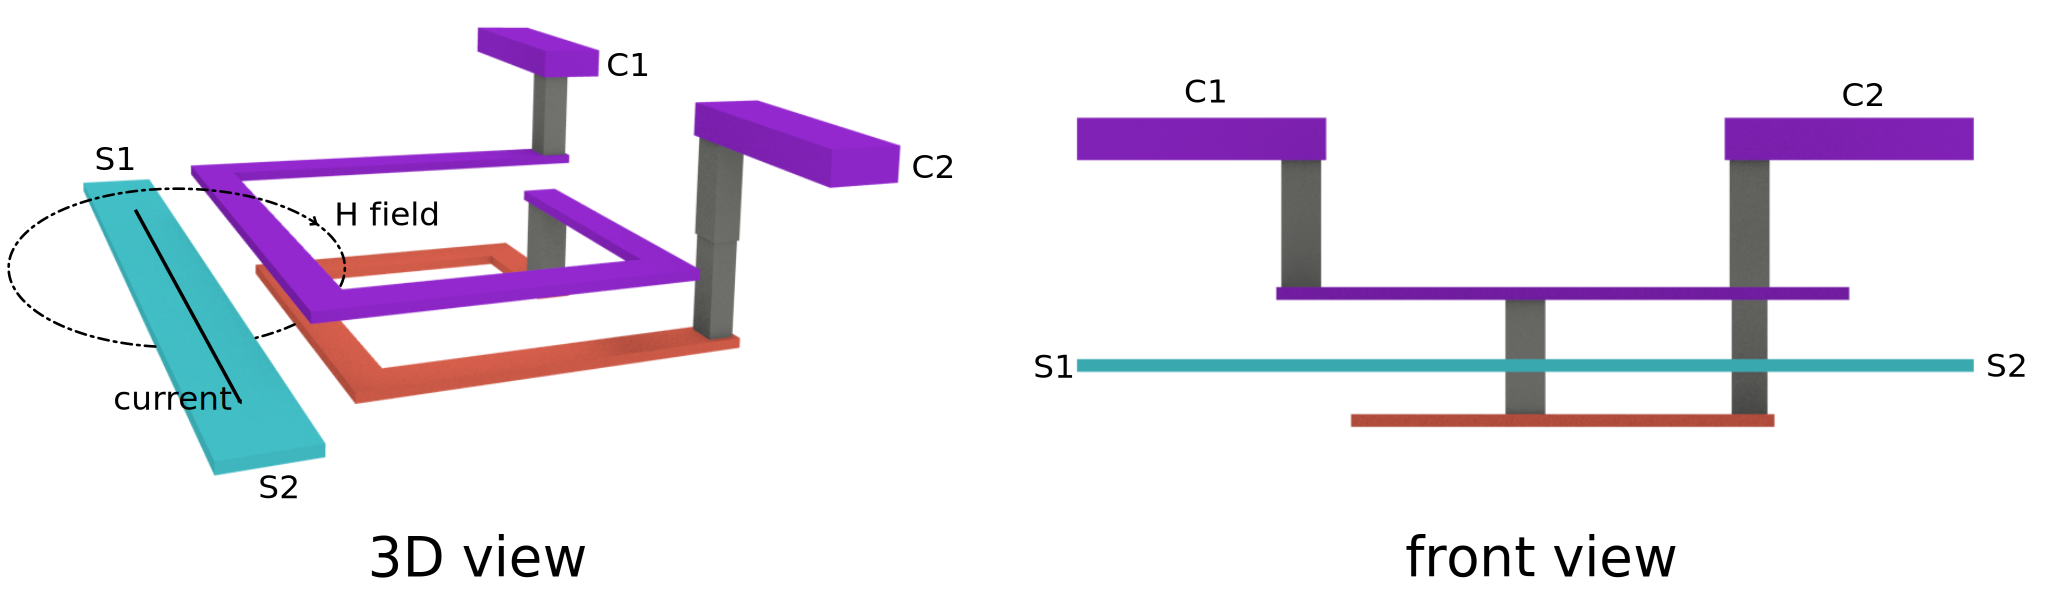
\includegraphics[width=0.98\textwidth]{src/3/figures/near-field-current-sensor.pdf}
  \caption{Near-field current sensor design}
  \label{fig:near-field-current-sensor}
\end{figure}

\begin{figure}[!h]
  \centering
  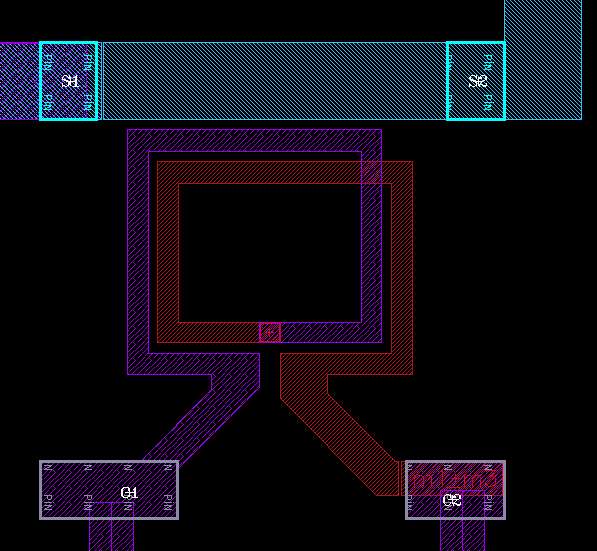
\includegraphics[width=0.5\textwidth]{src/3/figures/sensor_layout.png}
  \caption{Near-field current sensor layout}
  \label{fig:near-field-current-sensor-layout}
\end{figure}

% How is it designed and how is it used
On silicon, three levels of metal are used to build the loop.
The first level (in red) and the third level (in purple) form a circle.
Metallic vias connect both levels to close the loop vertically.
Finally, the sensed current is at the second level (pale blue), and circulates between nets \textit{S1} and \textit{S2}.
An oscilloscope with 50\textOmega{} input impedance performs a differential voltage measurement between pins \textit{C1} and \textit{C2}.
An example waveform obtained by injecting a rectangular pulse is given in Fig. \ref{fig:nfs-wvf}.
The obtained waveform requires specific post-processing to reconstitute the original current waveform.
The post-processing is detailed earlier in section \ref{sec:on-chip-near-field-process}.

\begin{figure}[!h]
  \centering
  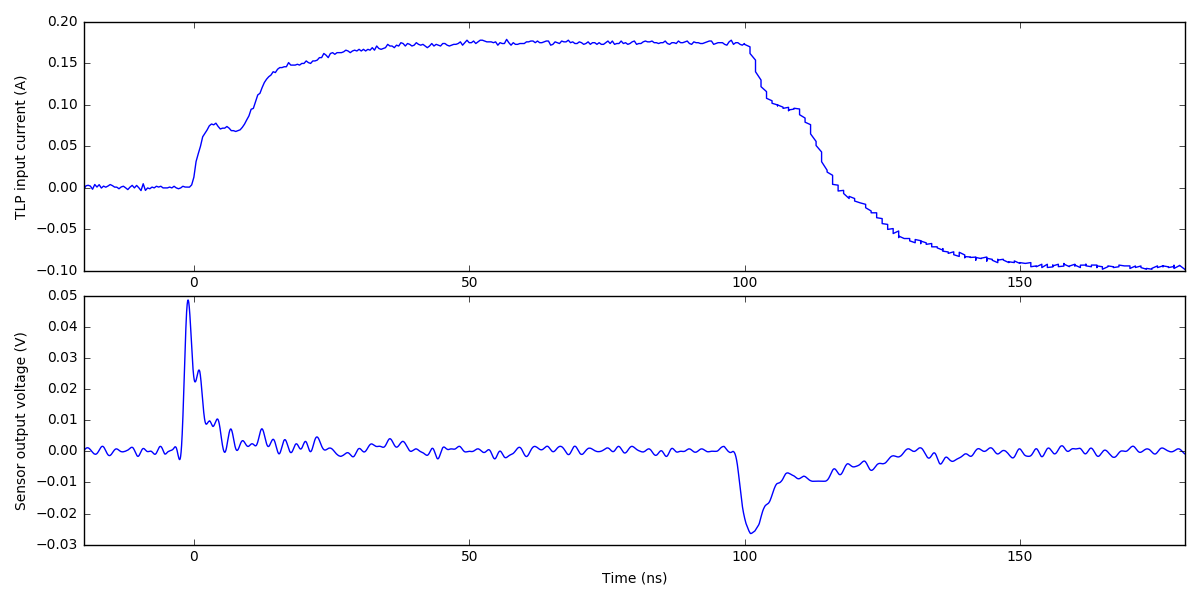
\includegraphics[width=0.9\textwidth]{src/3/figures/measured_waveform.png}
  \caption{Waveform measured with an oscilloscope connected to the on-chip near-field sensor}
  \label{fig:nfs-wvf}
\end{figure}

% Talk about the near-field current sensors placement
In total, there are 6 near-field current sensors located on the device.
The 6\textsuperscript{th} sensor is dedicated to calibration.
The others are placed strategically on main \gls{io} susceptible to be disturbed directly or indirectly by \gls{esd}s.
Sensor \textit{1} measures the current on the supply under test power input.
During testing, this pin is be exposed to \gls{esd}s coupled on top of a DC supply voltage.
Internally, this input is protected by a large \gls{esd-protection}, able to sustain IEC 61000-4-2 \gls{esd-gun} discharges.
Sensor \textit{2} measures the current absorbed and deviated by the \gls{esd-protection} into the \textit{gndsub} metal ring (local ground reference).
Sensors \textit{3} measures the current flowing to the external stabilisation capacitor of the regulator under test.
Finally, sensors \textit{4} and \textit{5} measure the currents flowing from the \textit{gndsub} metal ring into the external ground pins, connected externally to the board ground.

\subsection{Topcell}

%
The primary supply chain under test is directly extracted from a real product, described in \ref{sec:product-desc}.
It is placed in appropriate operating conditions on the testchip, and behaves identically to the real product.
Except for the two supply blocks, all the functionalities described previously were designed, simulated and layouted.
All layouts were assembled together to form the topcell (Fig. \ref{fig:top-cell-layout}).
The complete pinout is given in appendix \ref{apx:testchip-pinout}.

\begin{figure}[!h]
  \centering
  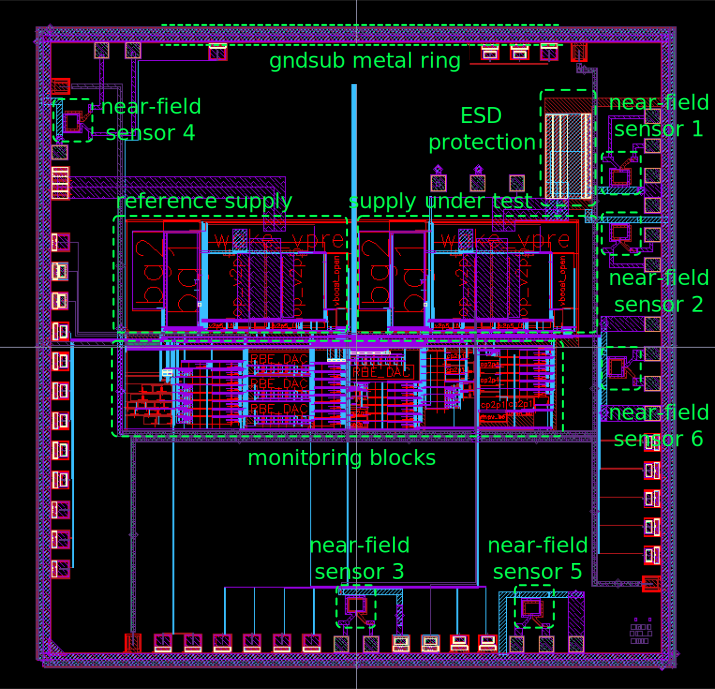
\includegraphics[width=0.7\textwidth]{src/3/figures/topcell_layout.pdf}
  \caption{Top-cell layout}
  \label{fig:top-cell-layout}
\end{figure}

% Explain why so much empty space
On the layout, a lot of silicon space was left empty.
This is due to manufacturing constraints that enforced the silicon dimensions.
After manufacturing and packaging, the chip is tested.
The entire testing process and results are documented in section \ref{sec:test-vehicle-testing}.
